\section{Historia}
\label{sec:historia}

Un dron no es más que una aeronave no tripulada que se controla remotamente y que, por lo general, se puede decir que siempre ha sido el sueño de todo estratega militar, ya que permite alcanzar al enemigo a distancia así como evitar pérdidas humanas.

Este sueño comenzó en el 1916, cuando el profesor Archibald Low, un militar científico, diseñó un torpedo aéreo que se manejaba con un sencillo control usando señales de radio. La aeronave fue un fracaso, pero sentó las bases para futuros diseños.

En Vietnam también se usaron otros modelos de dron como el Ryan Firebee que introdujo una nueva idea, la cámara de fotos para espiar al bando contrario.

\begin{figure}[H]
  \centering
  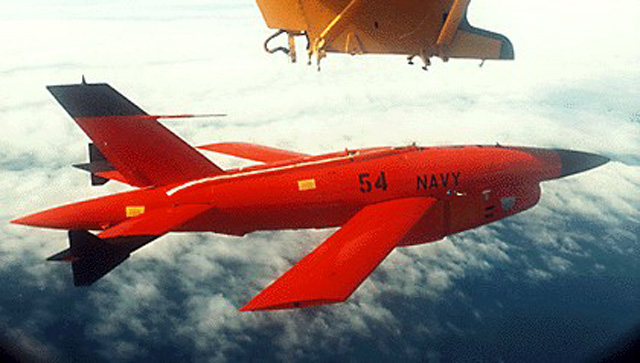
\includegraphics[scale=0.65]{imagenes/ryanfirebee.jpg}
  \caption{Ryan Firebee}
  \label{fig:ryanfirebee}
\end{figure}

Pero si hay que hablar de una salto en el desarrollo de los drones entonces es necesario mencionar al Gnat que fue desarrollado por General Atomics, un contratista de defensa de San Diego, California, EE. UU. que introdujo las cámaras de video y con esto empezó una nueva era en el mundo de los dron.

\begin{figure}[H]
  \centering
  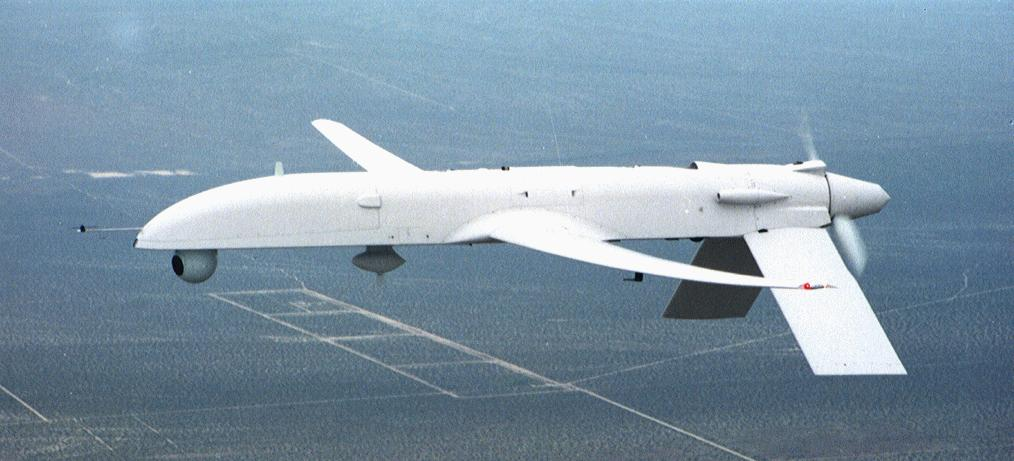
\includegraphics[scale=0.4]{imagenes/gnat.jpg}
  \caption{Gnat}
  \label{fig:gnat}
\end{figure}

Para comenzar a hablar del uso de los dron por el público sin duda hay que mencionar a Nikola Tesla quien patentó por primera vez un vehículo no tripulado controlado remotamente al que llamó teleautomation y que hoy es uno de los principios que rige el diseño de un dron.    

Sin duda ha sido un gran salto, por un lado muchos encuentran divertido el uso de los drone para fines personales y comerciales como la entrega de paquetes y otros proyectos de Amazon y Google mientras que otros critican fuertemente su uso en la guerra para bombardear a terroristas.

\section{Tipos de drones}
\label{sec:tiposdrones}

Como vehículo aéreo puede tener diferentes formas, bien tipo avión, tipo helicóptero o incluso formas muy diferentes. Pero los drones no son algo nuevo, el ejemplo más antiguo fue desarrollado después de la primera guerra mundial, y se emplearon durante la segunda guerra mundial para entrenar a los operarios de los cañones antiaéreos. Sin embargo, no es hasta poco más que a finales del siglo XX cuando operan los drones mediante radio control con todas las características de autonomía.

Algunos tienen sistema GPS que les permite volver al punto donde inició de su vuelo. En el futuro se espera que los drones vuelen solos, tomando sus propias decisiones, evitando chocar contra las personas y poder evitar los objetos.

La mayoría de los drones se manejan con radio control, pero pueden ser también manejados y programadas mediante una tablet o un smartphone.

Se utilizan para múltiples tareas, desde tareas de vigilancia, fotografía, retransmisiones televisivas, agricultura, ocio y muchas más tareas, ya que cada poco se descubre una nueva forma de utilizar los drones.
La clasificación es muy amplia, pero la primera clasificación podría ser en función del tipo de alas.

\begin{itemize}
\item Drones de Alas Fijas: Tienen alas fijas y son similares a un avión.
\item Drones MultiRotor: Suelen ser cuadricópteros (4 rotores con hélices) aunque los hay que tienen 6 (hexacópteros) o incluso 8 hélices. Dos hélices giran en el sentido de las agujas del reloj y las otras dos en el otro sentido, creando así la fuerza de empuje necesario para llevar al dron hacia arriba. Se pueden mantener en el mismo sitio sin varias la posición, gracias a sus giroscopios y estabilizadores, lo que es perfecto para sacar fotos y grabar vídeos.
\end{itemize}

\begin{figure}[H]
\centering
\subfloat[Alas fijas\label{fig:alasfijas}]{
  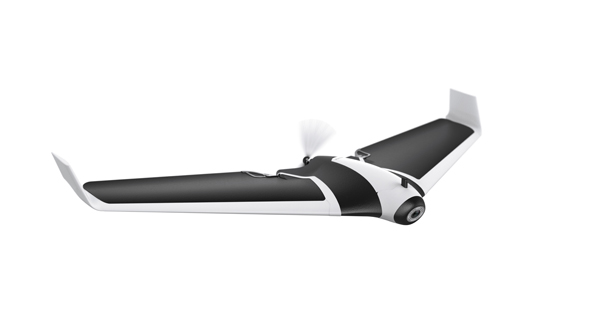
\includegraphics[width=.5\linewidth]{imagenes/parrot-disco.jpg}
}
\subfloat[Multirotor\label{fig:multirotor}]{
  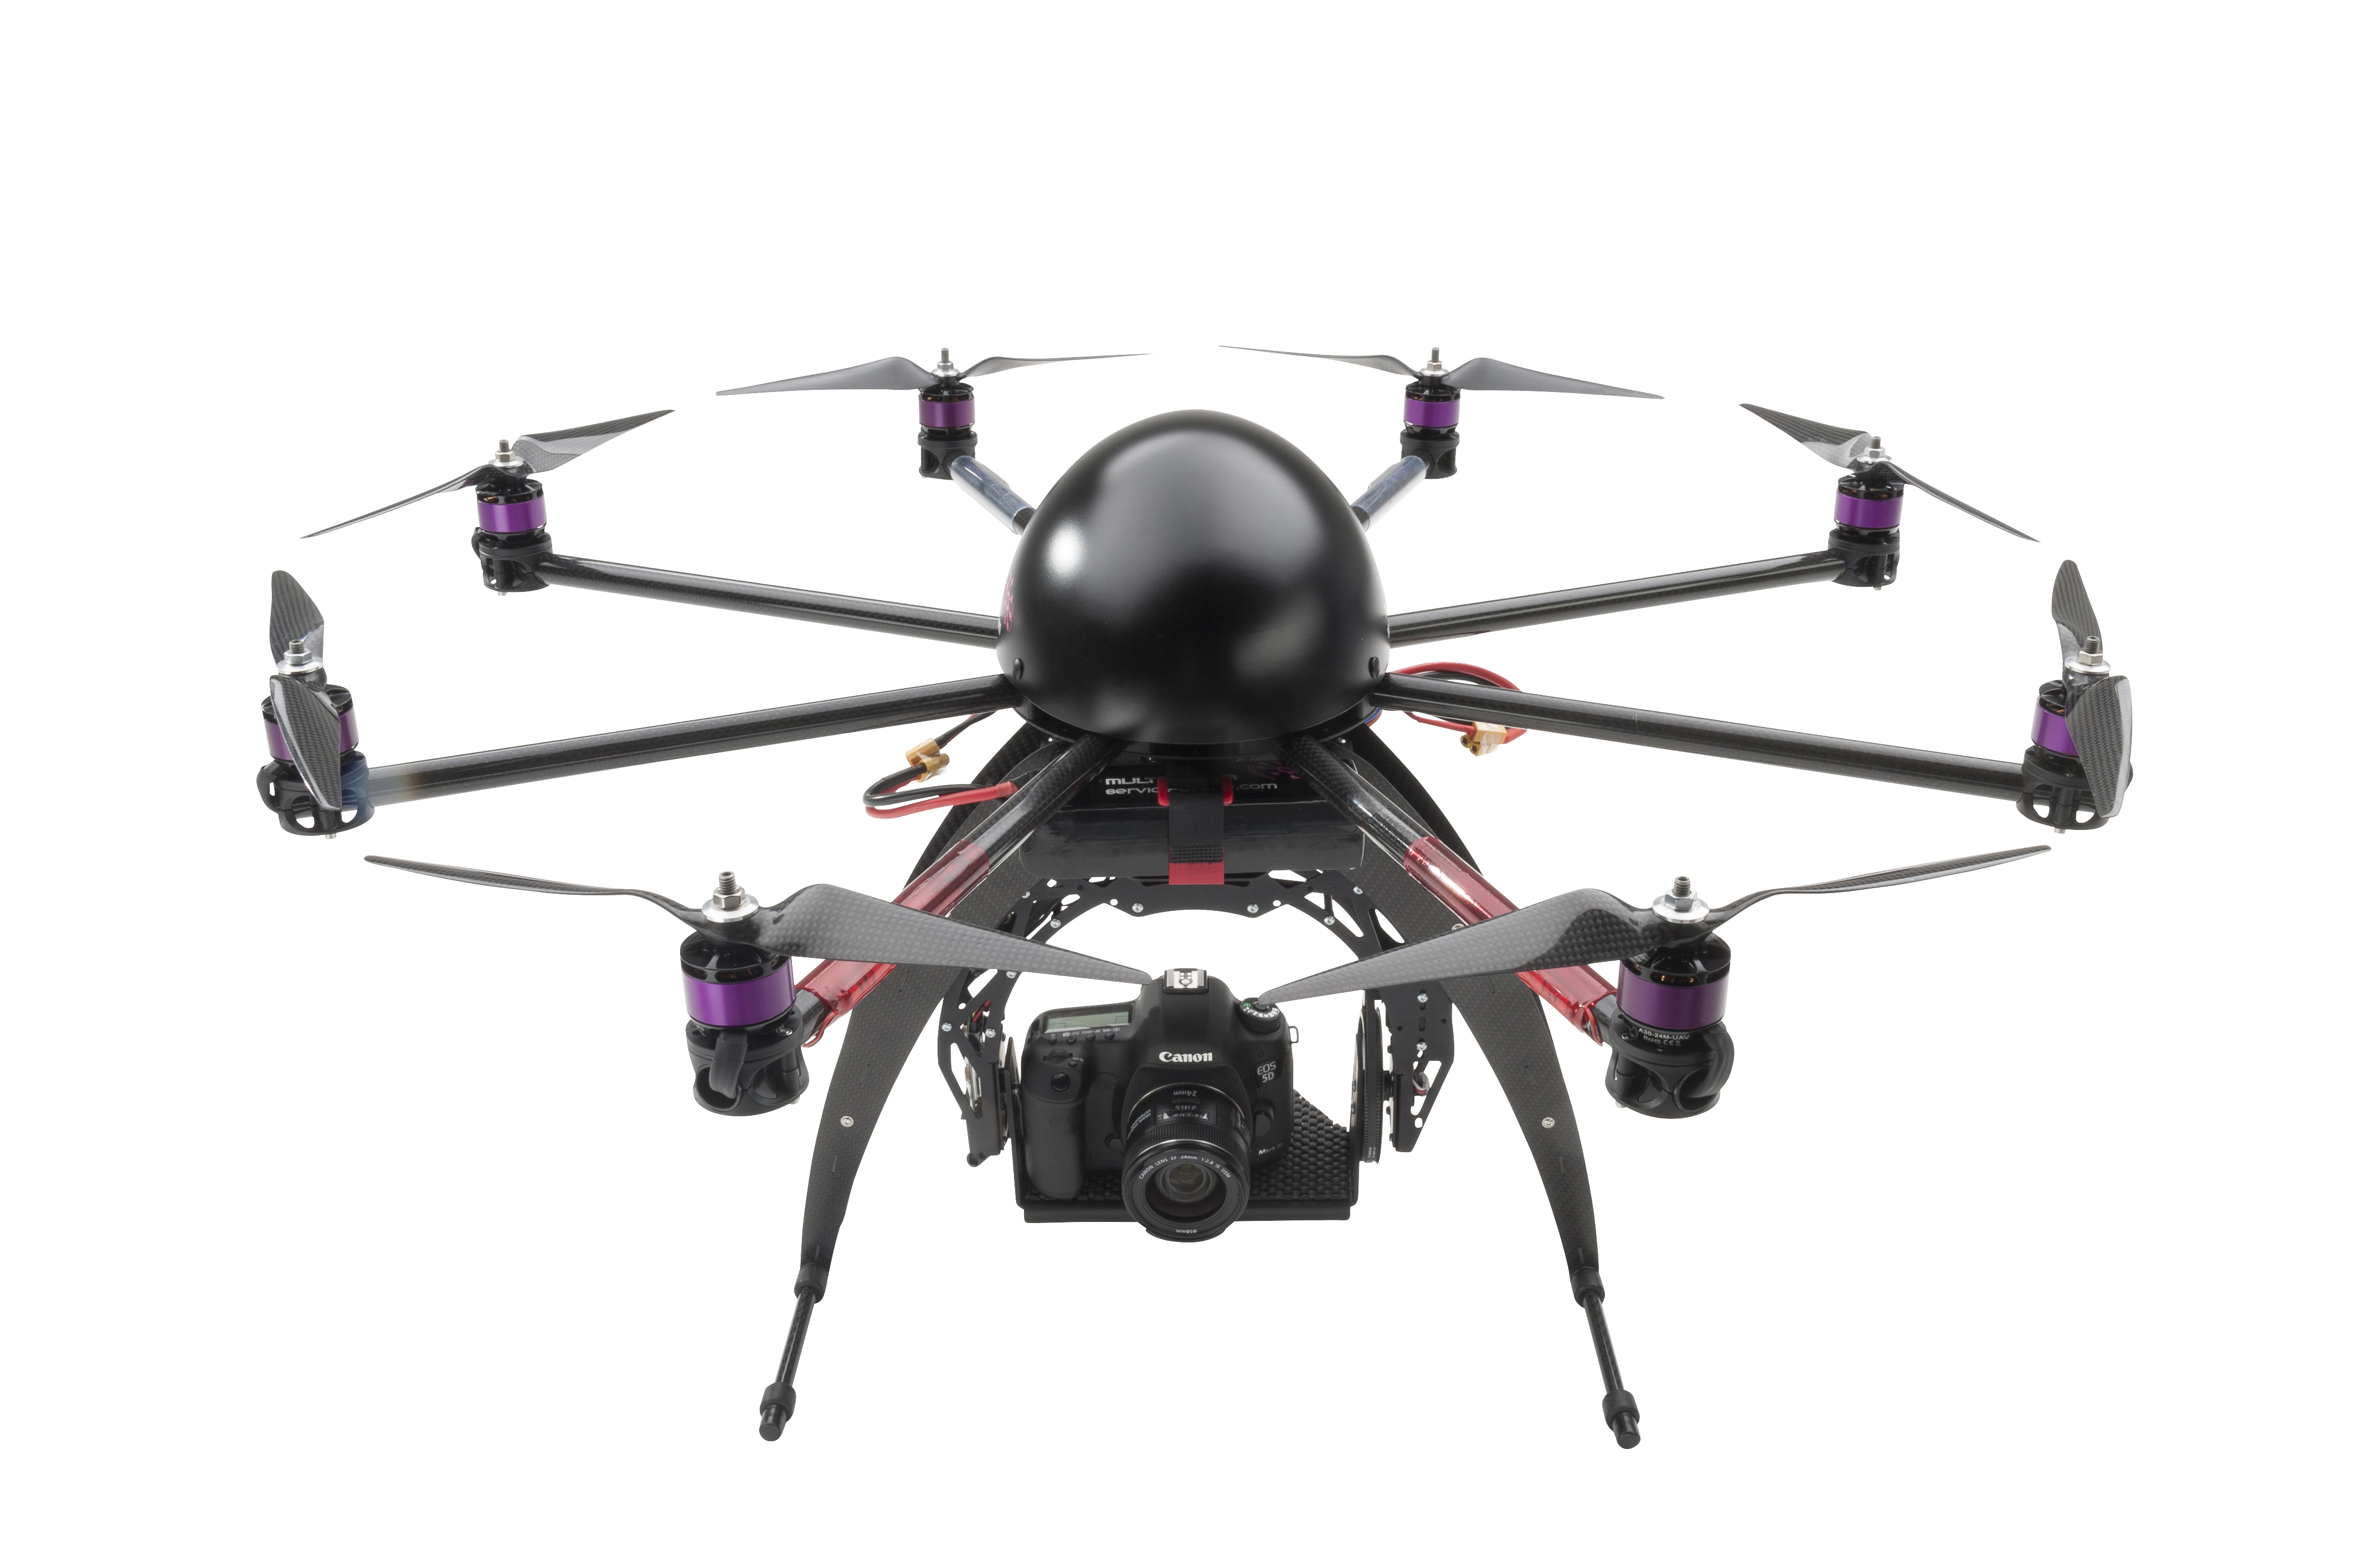
\includegraphics[width=.5\linewidth]{imagenes/multirotor.jpg}
}
\caption{Clasisficacion por alas}
\end{figure}

Según el método de control tenemos:

\begin{itemize}
\item Autónomo: El drone no necesita de un piloto humano que lo controle desde tierra. Se guía por sus propios sistemas y sensores integrados. 
\item Monitorizado: En este caso si se necesita la figura de un técnico humano. La labor de esta persona es proporcionar información y controlar el feedback del drone. El drone dirige su propio plan de vuelo y el técnico, a pesar de no poder controlar los mandos directamente, sí puede decidir que acción llevará a cabo.
\item Supervisado: Un operador pilota el dron, aunque este puede realizar algunas tareas autónomamente.
\item Preprogramado: El dron sigue un plan de vuelo diseñado previamente y no tiene medios de cambiarlo para adaptarse a posibles cambios.
\item Controlado remotamente(R/C): El drone es pilotado directamente por un técnico mediante una consola.
\end{itemize}

En función de su uso pueden ser:

\begin{itemize}
\item Drones Militares: son llamados UCAV que procede del ingles Unmanned Combat Air Vehicle, traducido al español sería vehiculos no tripulados de combate aéreo. Suelen ir armados y con capacidad de bombardeos.
\item Monitorizado: En este caso si se necesita la figura de un técnico humano. La labor de esta persona es proporcionar información y controlar el feedback del drone. El drone dirige su propio plan de vuelo y el técnico, a pesar de no poder controlar los mandos directamente, sí puede decidir que acción llevará a cabo.
\item Drones Civiles: son aquellos drones que no tienen uso militar. A su vez pueden ser de: \begin{itemize}
\item De uso comercial: como cartografías, fotografías, vídeos, etc.
\item Para Aficionados: Se utilizan como un juguete y suelen tener precios bastantes económicos.
\item Para Uso del Gobierno: Se utilizan para bomberos, fuerzas de rescate, etc. con el fin de ayudar a las tareas de reconocimiento, rescate, fronterizas e incluso fiscales.
\end{itemize}
\end{itemize}

\section{Aplicaciones}
\label{sec:aplicaciones}

Se pueden aplicar en ambientes de alta toxicidad química y radiológicos en desastres tipo Chernóbil, en los que sea necesario tomar muestras con alto peligro de vidas humanas y realizar tareas de control de ambiente. Las aeronaves cumplen con las normas regulatorias establecidas en el Tratado de Cielos Abiertos de 1992 que permiten los vuelos de VANT sobre todo el espacio aéreo de sus signatarios. Además, pueden cooperar en misiones de control del narcotráfico y contra el terrorismo. También podrían grabar vídeos de alta calidad para ser empleados como medios de prueba en un juicio internacional.

Los UAV tienen múltiples aplicaciones y posibilidades en el mercado civil y profesional:
\begin{itemize}
\item Internet: distribución de señal gratuita de internet.
\item Cartografía: realización de ortofotomapas y de modelos de elevaciones del terreno de alta resolución.
\item Monitorización de instalaciones.
\item Transporte y entrega de mercancías.
\item Agricultura: gestión de cultivos.
\item Cine y deportes extremos.
\item Servicios forestales: seguimiento de las áreas boscosas, control de incendios.
\item Búsqueda, rescate y salvamento de personas.
\item Medio ambiente: estado de la atmósfera.
\item Seguimiento de la planificación urbanística.
\item Gestión del patrimonio.
\item Seguridad y control fronterizo.
\item Purificar el aire mediante un proceso de filtrado mediante capas de poliéster y carbón activado en ambientes de la industria y el hogar. 
\end{itemize}

\begin{figure}[H]
\centering
\subfloat[Aplicación en agricultura\label{fig:dronagricultura}]{
  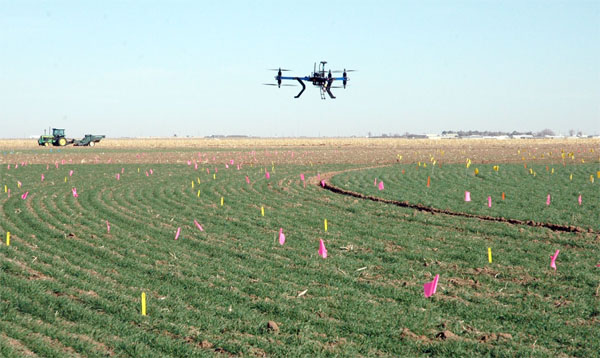
\includegraphics[scale=0.4]{imagenes/dron-agricultura.jpg}
}
\subfloat[Aplicación en transporte\label{fig:drontransporte}]{
  \includegraphics[scale=0.125]{imagenes/dron-paquete.jpg}
}
\caption{Clasisficacion por aplicación}
\end{figure}

\section{Normativa sobre Drones}
\label{sec:normativa}

En el documento oficial del Estado quedan reflejadas las condiciones en las que se puede realizar trabajos técnicos y científicos, tales como grabación aérea, reportajes aéreos, fotografía aérea, estudios de fotogrametría, vigilancia y monitoreo y revisión de infraestructuras entre otros. Gran parte de este nuevo decreto de ley temporal, se basa en 4 puntos clave que toda empresa que desee operar con drones deberá contemplar y seguir:

\begin{itemize}
\item Tipo de Drone
\item Espacio aéreo
\item Seguridad
\item Carnet de piloto de Drone
\end{itemize}

\subsection{Tipo de dron}
Se establecen dos categorías inciales: Drones con peso inferior a 2Kg. y drones con peso entre los 2Kg. y 25Kg. Para ambos es imprescindible disponer de un carnet de piloto de drones para poder operar en España.En caso de los drones de peso inferior a 2kg, no será necesario que estén inscritos en el registro de aeronaves ni disponer de un certificado de aeronavegabilidad.Para ambos tipos de drone, será necesario incluir obligatoriamente una placa identificativa con el nombre del fabricante del aparato así como los datos fiscales de la empresa que lleve a cabo dichas operaciones.

\subsection{Espacio aéreo}
El espacio aéreo pertenece a AESA, y como tal, para poder realizar cualquier tipo de actividad comercial o civil con un drone, se deberá obtener un permiso oficial, como mínimo 5 días antes de llevar a cabo cualquier operación en el aire. Esta nueva legislación sigue manteniendo la prohibición de sobrevolar núcleos urbanos o espacios con una alta masificación de gente sin el consentimiento especial por parte de la Agencia Española de Seguridad Aérea.

\subsection{Seguridad}
El pilar fundamental en el que se ha basado el Ministerio para la realización de la normativa de uso de drones civiles en España es la seguridad. Por ello cada empresa deberá disponer de un manual de operaciones cumplimentado siguiendo el estándar proporcionado por el Ministerio, así como un estudio de seguridad de cada una de las operaciones a realizar. Es decir, si alguien piensa en hacer volar un drone al margen de la ley, ya sea con un peso inferior a 2kg, o entre 2kg y 25kg, se expone a sanciones que van entre 3.000 a 60.000 euros.

\subsection{Carnet de piloto de Drones en España}
Para que las empresas puedan operar legalmente, como lo hace Dronair, los pilotos designados deberán disponer de un carnet oficial para el manejo de drones.. Si estos pilotos ya disponen de un título de piloto de avión, ultraligero u otro específico, no será necesario obtener dicha titulación. En caso contrario deberán cursar una serie de exámenes y pruebas oficiales para obtener el carnet oficial de piloto de drones. A día de hoy, no existen academias oficiales bajo la tutela del Gobierno que realicen estos cursos, por eso y mientras se empiezan a impartir estos cursos, será obligatorio demostrar que se dispone de los conocimientos teóricos y algún tipo de carnet oficial o documento que acredite a los pilotos en el manejo de drones para poder llevar a cabo cualquier operación.

\section{Hardware de drones}

Hay que destacar las partes que tiene un drone y su forma, pues es gran parte
lo que lo hace tan especial, permite que tenga una gran libertad de movimientos, ya
que puede moverse sin problema desde cualquier punto hacia los ejes X, Y y Z. Lo
que se gana con esto son funcionalidades como poder permitirse un aterrizaje y un
despegue totalmente vertical, sin depender de un espacio en el que coger velocidad
para levantar el vuelo, e igual con el aterrizaje, pudiendo el drone estando quieto en
el aire bajar totalmente en vertical hasta posarse sobre el suelo. Una vez en el aire
pueden moverse adelante, atrás, izquierda, derecha, arriba, abajo y combinaciones de
movimientos entre ejes, además de los giros Roll, Yaw y Pitch y sin necesidad de hacer
movimientos bruscos. Sin embargo, en los anteriores UAV solo tenemos el movimiento
hacia adelante, teniendo que jugar con Roll, Yaw y Pitch para poder movernos en los
distintos ejes.

\begin{figure}[H]
  \centering
  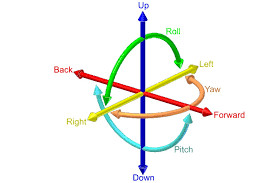
\includegraphics[scale=0.8]{imagenes/pitchRolYaw.png}
  \caption{Diferentes movimientos que puede realizar un drone.}
  \label{fig:gnat}
\end{figure}

Un desglose explicando cada una de las partes sería:
\begin{itemize}
\item Marco: También conocido como estructura o chasis. Es la estructura
principal sobre la que se sitúan el resto de los elementos. Cambiará su forma
dependiendo del drone, variando la longitud de las patas o el número de soportes
para hélices, por ejemplo. Puede estar hecha por diversos materiales, generalmente se
trata de algún tipo de plástico, ya que es un material que tiene poco coste y pesa poco.
Un ejemplo es el polipropileno, que es ligero y con mucha resistencia, lo que permite
colocar sobre él la batería. Otro material que suele utilizarse es la fibra de carbono,
ya que pesa poco y es muy resistente, aunque puede tener factores negativos como su
conductividad. Por último, también nombrar la fibra de vidrio. Este material también
es muy utilizado por ser ligero, y tiene características como que no es conductor de la
electricidad. Es común ver estructuras híbridas entre distintos materiales, sobre todo
juntando los dos tipos de fibra.
\item Hélices: Elemento formado por dos palas montadas de forma concéntrica
sobre un eje, que al girar crean un par de fuerzas, permitiendo así el movimiento del
drone.
\item Motores: Son los encargados de transformar la energía que llega en
movimiento sobre el eje en el que se sitúan las hélices, para así permitirles a éstas
hacer su trabajo. éste, a su vez, tiene distintos parámetros que serán principalmente
los que permitan al drone llevar mayor velocidad:
	\begin{itemize}
	\item El número de vueltas que dé por minuto, lo que dependerá de los KiloVoltios.
Suele estar en torno a 800-900kV.
	\item El tamaño que el drone tenga. Al mirar las especificaciones de un drone está en
un número de 4 dígitos, en el que los dos primeros hacen referencia al tamaño
del rotor y los otros dos al tamaño de la bobina.
	\item El empuje, valor que hacer referencia al peso que puede levantar el motor.
	\item La corriente, se trata de la energía (amperios) que se consume cuando el motor
está al máximo.
	\end{itemize}
\item Batería: Encargada de proporcionar la energía suficiente para que el drone
pueda realizar un vuelo, permitiendo trabajar a la placa controladora y motores. La
característica principal de las baterías son los miliamperios hora, ya que es la que
permitirá una mayor capacidad y por lo tanto que el drone tenga un mayor tiempo
de vuelo. Existen baterías de muy diversos tamaños, desde los 350 mah en drones de
juguete a, por ejemplo, los 4500mah que tiene la batería del drone 3DR Solo. También
es importante la tasa de descarga, que es la máxima energía que puede entregar y el
periodo de tiempo durante el que puede hacerlo. Normalmente los drones traen sistemas
de alerta que avisan cuando a la batería le queda poca energía, o que cuando queda
un valor menor a cierto porcentaje de carga no permite despegar el drone, evitando así
que se quede sin energía a mitad de un vuelo.
\item Equipo de transmisión: Es el encargado de que se comunique el drone con
una estación receptora. Puede variar en función del aparato ya que se pueden usar
diferentes tecnologías, pero principalmente usa radiofrecuencia o Wifi. Existen casos,
como el modelo 3DR, que combina ambas tecnologías, utilizando la radiofrecuencia
para la información del movimiento, batería y posicionamiento, y el WiFi para la
transmisión de imágenes en directo. Se pueden encontrar distintos equipos de sistemas
de transmisión, uno de los últimos y más destacables es Hyperion, que utiliza un
sistema óptico de comunicaciones capaz de transmitir hasta 1Gb por segundo, lo que
permite la transmisión de datos mediante la luz directa. Su principal característica
es que no pierde información cuando no hay contacto directo entre las dos estaciones.
La vía WiFi es muy utilizado, pues permite controlar el drone desde una aplicación
móvil, por lo que conectando estos dos tendríamos un mando que nos permite cambiar
gran parte de la configuración del drone. También existen dispositivos que permiten
el control mediante Bluetooth, pero es menos común ya que tiene mayor restricción de
velocidad de datos y distancia.
\item Placa controladora: Es el procesador del drone, el que se encarga de recoger
la información del drone y cuando le llega una orden ver que información tiene que
mandar para que ésta se ejecute de forma correcta, así como en caso de haber un
problema tratar de evitarlo. Hay una gama muy amplia:
	\begin{itemize}
	\item Pixhawk2: Es el más utilizado debido a que trabaja con 3DRobotics y Ardupilot.
Sirve para diversos dispositivos como drones, helicópteros y barcos. Está pensado
para cualquier vehículo que tenga movimiento. Se trata de un proyecto hardware
abierto, cuyo objetivo principal es proporcionar el hardware de autopiloto a
comunidades académicas o gente que tiene esto como un hobby, teniendo así
un bajo costo y una alta disponibilidad. Es un piloto automático en tiempo real
y muy eficiente, proporcionando un entorno de estilo POSIX. éste es el autopiloto
estándar de la industria, y por lo tanto, como veremos a continuación, a partir
él se han desarrollado diversos autopilotos con distintas mejoras.
	\item Pixhawk2: Es una versión avanzada de la placa anterior. Tiene mejoras
como aislamiento de vibraciones, 3 IMUs para redundancia (3 acelerómetros,
3 giróscopos, 3 magnetómetros y 2 barómetros) y sensor para controlar la
temperatura.
	\item PixRacer: Se ha desarrollado para los drones de carreras, aunque también se
utiliza en minidrones. Suele tener una mayor memoria flash.
	\item Navio2: Piloto automático diseñado de Raspberry Pi. Te permite convertir ésta
en un controlador de drone.
	\item PXFmini: Es otro piloto automático de Raspberry Pi. éste tiene la electrónica
para la mayoría de los componentes que puede utilizar un drone.
	\item FlytPOD: Es una placa Odroid XU4 SBC junto con una PixHawk. Puede
volar diversos vehículos aéreos y su principal característica es el WiFi que tiene
integrado. Existe una placa FlytPOD pro que es una versión extendida de la
anterior, con más sensores y mayor capacidad de almacenamiento.
	\item U-Pilot: Este hardware se caracteriza por servir para diversos vehículos aéreos,
siendo programable para realizar todas las acciones de su camino de forma
automática. Su radioenlace con frecuencia en torno a 900Mhz permite controlar
el dispositivo a una distancia de 100km.
	\end{itemize}

\end{itemize}

Hay que destacar un elemento importante como es la cámara, que aunque no
todos los drones la llevan sí es bastante común. Algunos la llevan incorporada (incluso
dos cámaras, una que apunta hacia la parte de delante y otra que apunta la parte
de abajo) y otras que traen soporte para incorporar ciertas cámaras, normalmente
consideradas cámaras de acción, para obtener una mejor calidad. Algunos drones
incorporan una Gimbal para controlar la parte hacia la que queremos que apunte la
cámara en cada momento o utilizarlo como estabilizador, para evitar así que afecten a
la imagen diversos movimientos, generalmente bruscos, que pueda realizar el drone.
En ocasiones, utilizado normalmente para carreras de drones, la cámara sirve
para integrar la tecnología FPV (First Person View), que es junto a la cámara, el
transmisor de vídeo y el receptor de vídeo, poder ver en tiempo real las imágenes sobre
una pantalla LCD o utilizando unas gafas de realidad virtual. En esta linea uno de los
sistemas más impactantes es el conjunto que se ha creado con el done FLYBi, estando
éste conectado a unas gafas de realidad virtual que tienen sensor de movimiento, lo que
te permite sentir que eres tú el que vuelas y el que estás en el lugar del drone, y con
cualquier movimiento que sientan las gafas la cámara del drone lo imitará. En caso de
que esto parezca incómodo tiene un joystick con el que también se pueden ordenar los
movimientos realizar a la cámara.

\begin{figure}[H]
  \centering
  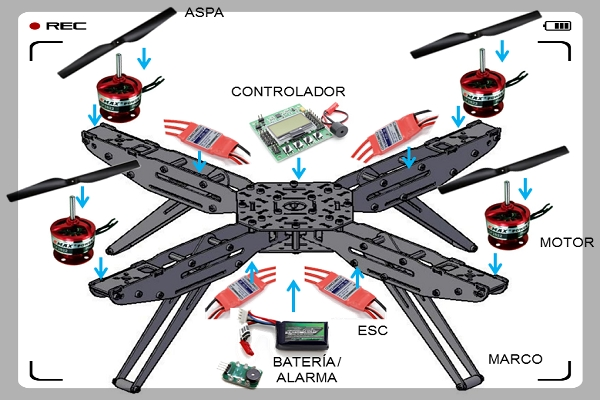
\includegraphics[scale=0.8]{imagenes/partesdron.jpg}
  \caption{Distintas partes de un dron.}
  \label{fig:gnat}
\end{figure}

\section{Software de drones}

El software es el conjunto de programas que permiten realizar ciertas tareas, por
ejemplo al drone una navegación autónoma. Dicho programa estará instalado en la
placa controladora, y por tanto será el que ejecute para recoger la distinta información
de los sensores, procesar la información y enviar las órdenes correctas a los distintos
elementos. El desarrollo de software para este tipo de robots ha evolucionado mucho
en los últimos años debido al uso civil que se le comienzan a dar y no tanto al desarrollo
militar. Existen varios entornos software que permiten el manejo y la programación de
estos robots:
\begin{itemize}
\item Ardupilot3: Es un sistema OpenSource encargado de recibir la información
que se le da y de enviar las señales correspondientes a los actuadores. Se
trata del software más importante por lo completo que es y la confiabilidad que
proporciona, debido a la gran cantidad de gente que lo utiliza (pilotos de drones
profesionales y aficionados) y por el equipo de ingenieros que lo han desarrollado.
Este software se caracteriza por la variedad de dispostivos que puede llegar a
controlar, ya que trabaja con diversos dispositivos aéreos (aviones, helicópteros,
drones, etc) y con dispositivos marinos (como son los barcos y submarinos). éste
ha tenido un gran desarrollo debido a que es código abierto. Hay mucha gente
creando interfaces para él y dichos usuarios comparten sus avances con el resto.
A partir de éste han nacido controladores como Ardupilot Mega. El problema
que tiene dicho software es que sólo permite trabajar con plataformas de los
mismos creadores. Otra característica es la facilidad con la que se le pueden
añadir diferentes sensores, como pueden ser módulos GPS o cámaras, algo que
facilita la navegación autónoma.
\item Megapirate-NG: Apareció como desarrollo del anterior. La funcionalidad de
uno y otro es prácticamente la misma, con la diferencia de que éste permite
trabajar con Hardware de otros creadores. El problema es que siempre depende
de Ardupilot, por lo tanto sus funcionalidades, aunque sean más cómodas para
trabajar, puede que estén atrasadas.
\item MultiWii: Se propuso como radiocontrol para drones. Es un sistema que fue
creado por los desarrolladores y con los sensores (giroscopios y acelerómetros) de
la Nintendo Wii. Es una plataforma basada en arduino, con el factor en contra
de tener una funcionalidad bastante limitada.

\end{itemize}

Estos son los entornos software principales que estarían sobre el vehículo, pero
también están los programas que se ejecutarían en otros dispositivos como el ordenador
o el teléfono móvil para ver la información que éste nos envía. Normalmente el
fabricante del drone tiene ya un programa que realiza esta función.
En este punto es importante el protocolo de comunicación que habrá para
comunicar el vehículo con la estación terrena. Aquí hay un protocolo que destaca
sobre los demás, el MAVLink (Micro Air Vehicle Communication Protocol). Este
protocolo tiene la información contenida en ficheros .xml, lo que permite utilizarlo en
diversos lenguajes de comunicación, y conlleva una mejora notable en su desarrollo. Al
tener el fichero .xml los tipos de mensaje, permite con facilidad añadir nuevos tipos
para asignar una tarea nueva. Otra ventaja es que hay muchos software de drones
que lo soportan, como pueden ser Ardupilot, Autopilot, algunos derivados de éstos y
otros como Gentlenav o Flexipilot, y desde la estación tierra algunos como MAVProxy,
Mission Planer o APM planner. Un problema en este protocolo es que los datos no están
encriptados en la comunicación, por lo que es más fácil un ataque y que se manipulen
los datos. Además detecta si se pierde algún dato ya que utiliza CRC (código de
redundancia cíclica para detectar cambios en los datos, este se utiliza en protocolos
como TCP). MAVLink utiliza otro software llamado MAVProxy para acceder a los
datos del vehículo, como la velocidad y las imágenes, lo que permite también saber qué
datos mandarle para que funcione de forma correcta.
Destacar ROS (Robot Operating System), meta sistema operativo de código
abierto mantenido por la Open Source Robotics Fundation(OSRF). ROS tiene librerías
y herramientas que permiten desarrollar software para robots. Es el software para
robots más extendido en el mundo, lo que conlleva que sea el que más aplicaciones
tiene para la robótica. También ofrece mucho software para el manejo de drones. En
mayo de 2010 mostró el primer vídeo en el que un drone conseguia volar utilizando
ROS. En esta demostración el drone se movía con trayectorias agresivas, para mostrar
su correcto funcionamiento. Desde entonces ha seguido sacando herramientas para
ver el estado del drone conectando con los sensores, imágenes de las cámaras o GPS.
PIXHAWK también integró su sistema con ROS, lo que hizo que éste todavía creciera
más. También tiene interfaz para el control del ArDrone. Por otro lado, en protocolos
de comunicación MAVLink lanzó también un software para la compatibilidad con ROS.
A parte de todos éstos, existen también otras infraestructuras software como
JdeRobot, que es la que hemos usado en este trabajo y que se describirá con más detalle
en el capítulo 3.

\section{Robótica aérea en RoboticsLab de la URJC}
En un contexto más cercano, este proyecto se inició tras otros realizados
anteriormente en el laboratorio de robótica de la universidad. Los ejemplos más
destacables son los siguientes:
\begin{itemize}
\item Alberto Martín \footnote{\url{http://jderobot.org/Amartinflorido-tfg}} trabajó en el seguimiento de objetos con un drone
utilizando su cámara. Tenía un controlador reactivo PID, y el drone tenía que seguir una pelota de color rosa, consiguiendo que le siguiera en un espacio 3D. El drone en caso de no encontrar la pelota rosa se quedaba parado donde estuviera. Adicionalmente en este proyecto se desarrollo el driver para el ArDrone del Parrot real, que es el mismo que hemos utilizado en este proyecto.

\item Arturo Velez \footnote{\url{http://jderobot.org/Avelez-tfg}} trabajó en un seguimiento visual pero sin filtro de color,
en el cual un drone debe seguir una textura que se mueve por el suelo detectando los puntos de interés. En caso de que el drone pierda la referencia de la figura en la imagen, realiza un algoritmo de búsqueda.

\item Manuel Zafra \footnote{\url{http://jderobot.org/Mazafrav-pfc}} trabajó en la localizacion del drone mediante April Tags.
El objetivo de éste era recorrer autónomamente una ruta tridimensional en interiores,
como secuencia de puntos 3D para lo que necesitaba estar localizado. Gracias a las
April Tags que detectaba el drone podía detectar el punto en un mapa 3D en el que
estaba situado.

\item Danuel Yagüe \footnote{\url{http://jderobot.org/Daniyague-pfc}} trabajó con el ArDrone sobre Gazebo, probando distintas
funcionalidades y escenarios. Por un lado trabajó en el driver para el cuadricoptero
simulado, consiguiendo un plugin para el ArDrone que proporciona los datos de los
sensores a bordo y que acepta y ejecuta ordenes como despegar, aterrizar y los distintos
movimientos de vuelo. Por otro lado sobre simulador programó aplicaciones de control
visual, haciendo que el drone siguiera una linea, una carretera o que un drone siguiera
al otro.

\item Jorge Cano \footnote{\url{http://jderobot.org/J.canoma-tfg}}trabajó en el diseño, construcción y programación de un
drone real. El driver que realizó para su control se basa en el protocolo MAVLink, en
parte por su gran popularidad. Por una parte trabajó en el diseño y construcción de
la plataforma hardware, como se muestra en las dos primeras imágenes de la figura
1.13, y por otra en el contolador software para la comunicación con el vehículo. Para
hacer tests de vuelo realizó pruebas perceptivas y de control, con filtros de colores y
un controlador PID.
\end{itemize}

Una vez terminada la breve introducción, se va a explicar lo realizado en
este proyecto. En el capítulo 2 se redactan los objetivos propuestos y la metodología
seguida para llegar hasta ellos. En el capítulo 3 se presenta la infraestructura utilizada
y como se ha trabajado con ella. En el capítulo 4 se describe el driver que se ha implementado,
cómo se ha programado y porqué se han seguido unos u otros caminos. En el capítulo
5 se detalla la herramienta de apoyo para dirigir el dron y los resultados que se han obtenido.
Por último, en el capítulo 6 se incluyen las conclusiones a las que se han llegado tras
finalizar este proyecto.